\documentclass[12pt]{article}
\usepackage[utf8]{inputenc}
\usepackage{amsmath}
\usepackage{amsfonts}
\usepackage{graphicx}
\usepackage[backend=biber, style=apa]{biblatex}
\addbibresource{Bibliography.bib} 
\usepackage{hyperref}
\usepackage[spanish]{babel}
\usepackage{csquotes} % para citas adecuadas
\DeclareLanguageMapping{spanish}{spanish-apa} % mapeo del idioma

\begin{document}
	\begin{titlepage}
		  \centering
		 
		  
		  {\scshape\LARGE Facultad de Matemática y 
		  	Computación
		  	Universidad de La Habana\par}
		  \vspace{1cm}
		  
		   %\includegraphics[width=0.15\textwidth]{logo_universidad} % Logo de la universidad
		   \vspace{1cm}
		  
		  {\scshape\Large Tesis de diploma de la 
		  	Especialidad Ciencia de la 
		  	Computaci\'on \par}
		  \vspace{1.5cm}
		  
		  {\huge\bfseries Segmentaci\'on de \'Ulceras de Pie Diab\'etico (UPD) en secuencias de im\'agenes RGB mediante el Segment Anything Model (SAM). \par}
		  \vspace{2cm}
		  
		  {\Large Autor: Abdel Fregel Hern\'andez \par}
		  
		  \Large Tutor: Dr. Jos\'e Alejandro Mesejo Chiong
		  \vfill
		  
		  {\large La Habana}
		  
		  {\large \today \par} % Fecha actual
	\end{titlepage}
	
	\section{Agradecimientos}
	\pagenumbering{roman}
	\newpage
	
	
	\section{Resumen}
	\newpage
	
	\section{\'Indice}
	\tableofcontents
	\newpage
	\cleardoublepage
	\pagenumbering{arabic}
	
	
	\section{Introducci\'on}
	La dibetes(diabetes mellitus), es una enfermedad cr\'onica que afecta la forma en la que el cuerpo utiliza la glucosa, una fuente clave de energ\'ia. De acuerdo a la \textit{Federaci\'on Internacional de Diabetes}, en el a\~no 2021 se reportaron 6.7 millones de muertes a causa de esta enfermedad \parencite{DiabetesAtlas2024}. En nuestro pa\'is, seg\'un el \textit{Anuario Estadístico de Salud 2022} \parencite{msp2022}, la prevalencia es de 66,50\textdiscount de enfermos por cada 1000 habitantes.
	\\
	
	Cerca del 86\textdiscount \space de personas que padecen de diabetes sufren de \'ulcera de pie diab\'etico \footnote{Hace referencia a una complicaci\'on grave de la diabetes que se manifiesta como una herida o llaga abierta en el pie}(UPD), y corren el riesgo de amputaci\'on. La duraci\'on de estas pueden variar, algunas pueden durar semanas, sin embargo otras pueden tardar a\~nos. La calidad de vida de los pacientes que enfrentan esta situaci\'on se ve deteriorada.  En la actualidad, los médicos cubanos especializados en el tema no cuentan con una herramienta cuantitativa efectiva que valore la severidad y el proceso de curación de las UPD. La medición regular de las úlceras ayuda a evaluar la efectividad del tratamiento y a realizar ajustes según sea necesario. Un seguimiento adecuado puede prevenir la progresión de la úlcera y reducir el riesgo de amputaciones.
	\\
	
	Para resolver este problema se han hecho difrerentes estudios con el objetivo de realizar la medici\'on precisa de las UPD.
	El principal indicador de mejor\'ia de estas heridas es la disminuci\'on gradual del \'area y el per\'imetro, asi como de su volumen. Otro factor importante en el tratamiento de estas son la evaluación de la cicatrización y la regeneración del tejido. La formación de tejido granuloso sano es un indicador positivo, su presencia indica que el proceso de curación está en marcha \parencite{molnlycke2023}. La ausencia de signos de infección, como tejido necr\'otico, es un indicador clave de mejora. El control adecuado de infecciones contribuye a un entorno propicio para la cicatrización. 
	\\
	
	En este trabajo, para la tarea de segmentar las im\'agenes, utilizaremos una herramienta desarrollada por Meta AI llamada Segment Anything Model(SAM)\parencite{segmentanything2023} que permite identificar y segmentar objetos en imágenes de manera eficiente. Esta herramienta ha ganado popularidad en cuanto a las tareas de segmentaci\'on. Por lo tanto en el presente trabajo se estar\'a usando para hacer una segmentaci\'on de las imagenes de UPD.
	
	\subsection{Objetivos}
	Este trabajo tiene como objetivo desarrollar una herramienta que pueda, a trav\'es de una secuencia de im\'agenes RGB-D \footnote{RGB-D, se refiere a una camara capaz de captar im\'agenes a color(RGB, formato Red(rojo),Green(verde),Blue(\'azul) y un sensor de profundidad (D(depth),por su sigla en ingl\'es)}, hacer una medici\'on de la \'ulcera y de los tejidos que la componen para facilitar al doctor su tratamiento. Con esto en mente en esta tesis se propone un sistema que automatiza la segmentaci\'on a partir de las im\'agenes.
	\\
	
	
	Para lograr este objetivo general se tiene los siguientes objetivos espec\'ificos:
	
	\begin{itemize}
		\item[1] Hacer un estudio de la literatura sobre los m\'etodos de segmentaci\'on
		\item[2] Estudiar sobre la utilizaci\'on del Segment Anything Model.
		\item[3] La creaci\'on de un dataset para la posterior evaluaci\'on del modelo
		\item[4] La evaluaci\'on del modelo en cuanto m\'etricas de calidad. 
	\end{itemize}
	
	\subsection{Estructura de la tesis}
	Esta tesis cuenta con un total de 4 Capítulos. En el Capítulo 1 se expone
	la revisión de la literatura donde se presentan algunos de los algoritmos existentes, as\'i como datasets existentes. El Capítulo 2 hace una breve introducci\'on a SAM y a SAM para im\'agenes m\'edicas. El Cap\'itulo 3 explica la estructura y detalles de implementaci\'on de la propuesta final. Luego, en el Cap\'itulo 4 se muestra los resultados alcanzados y la comparaci\'on con otros modelos existentes, haciendo uso de las medidas de calidad. Finalmente se dan las
	conclusiones y recomendaciones de la investigación con el propósito de su
	futura continuación.

	
	
	
	\newpage
	
	\section{Cap\'itulo 1}
		\subsection{Estado del arte}
	
	
	\newpage
	
	\section{Cap\'itulo 2}
		\subsection{Segment Anything Model(SAM)}
		SAM utiliza una arquitectura transformer-based, la cual ha sido probada su eficiencia en el procesamiento de lenguaje natural y en tareas de reconocimiento de im\'agenes. Espec\'ificamente, SAM contiene un codificador de imagen(image encoder) basado en un Vision Transformer(ViT), con este extrae las caracter\'isticas de la imagen, tambi\'en utiliza un prompt encoder para integrar las interacciones del usuario y por \'ultimo un mask decoder con el objetivo de predecir las m\'ascaras de segmentaci\'on con la fusi\'on de las caracter\'isticas de la imagen con las entradas del usuario.
		
		\begin{figure}[h] 
			\centering
			\caption{ Imagen adaptada de}
			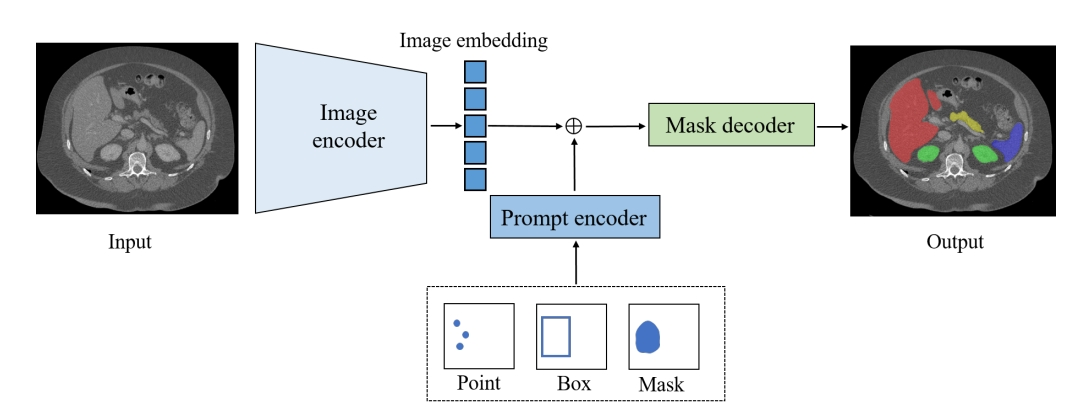
\includegraphics[width=1\textwidth]{1.jpeg}
			
			\label{fig:fig1}
			
			
		\end{figure}
	
	\newpage
	
	\section{Conclusiones}
	\newpage
	
	\section{Recomendaciones}
	en la figura \ref{fig:fig1}
	\newpage
	
	\section{Bibliograf\'ia}
	\printbibliography[title={" "}]
	\newpage
	
	\section{Anexos}
	
	
\end{document}